%% SafeStream-Redactor -- journal manuscript (Elsevier elsarticle, numbered references)
%% Target: Computers & Security. Self-contained: the bibliography is embedded below
%% (thebibliography), so no .bib file or BibTeX run is needed.
%% Compile with pdfLaTeX. Figures required in the same folder:
%%   fig_architecture.pdf, fig_memory.pdf, fig_accuracy.pdf, fig_scaling.pdf
\documentclass[preprint,12pt]{elsarticle}

\usepackage{amsmath,amssymb,amsthm}
\usepackage{booktabs}
\usepackage{graphicx}
\usepackage{xcolor}
\usepackage{algorithm}
\usepackage{algpseudocode}
\usepackage{tikz}
\usetikzlibrary{arrows.meta,positioning,fit}
\usepackage{xurl}
\usepackage[hidelinks]{hyperref}
\emergencystretch=3em

\newtheorem{theorem}{Theorem}
\newtheorem{assumption}{Assumption}
\renewcommand{\theassumption}{A\arabic{assumption}}
\newtheorem{definition}{Definition}
%% author-only information that must be supplied before submission
\newcommand{\MISSING}[1]{\textcolor{red}{[MISSING: #1]}}

\journal{Computers \& Security}

\begin{document}

\begin{frontmatter}

\title{Bounded-memory streaming redaction of personal data and credentials with a whole-document equivalence guarantee}

\author[aff1]{Mounish Senisetty\corref{cor1}}
\ead{senisettymounish@gmail.com}
\author[aff1]{\MISSING{co-author full name, or delete this line}}
\author[aff1]{\MISSING{co-author full name, or delete this line}}
\cortext[cor1]{Corresponding author.}
\affiliation[aff1]{organization={\MISSING{Department, Institution}},
            city={\MISSING{City}},
            country={\MISSING{Country}}}

\begin{abstract}
Logs, database exports and packet captures that leave an organisation carry personal data and credentials that must be removed first, and they are often too large to hold in memory. Processing them in chunks adds a failure mode that leaves no trace: a value straddling a chunk boundary reaches the detector in two halves, matches nothing, and is written out in the clear. We present SafeStream-Redactor, a local redaction engine that treats chunking as a correctness problem. Under two stated locality assumptions, bounded span length and bounded context, we show that its streamed output equals a whole-document pass, that its multi-process output equals the sequential output or falls back to it, and that its working buffer is independent of input size; the constants are derived from detector declarations and enforced at run time. These properties remove chunking as a source of leaks; they do not make detection complete. Measured peak memory added by streaming stayed below 8.6\,MiB from 8\,MiB to 2\,GiB of input, against 904.6\,MiB for whole-document redaction of the same 32\,MiB input. On held-out test splits the pattern tiers fully redacted more credentials than gitleaks and TruffleHog in default configurations (0.437 against 0.311 and 0.270). With the same spaCy model, SafeStream exceeded Presidio in character F1 (0.702 against 0.650). Document-level protection remains weak: no evaluated configuration redacted every must-redact character in more than 17.9\% of RedactionBench documents, and two of the three corpora are synthetic.
\end{abstract}

\begin{keyword}
data redaction \sep secret detection \sep data loss prevention \sep streaming algorithms \sep bounded memory \sep personally identifiable information
\end{keyword}

\end{frontmatter}

%% ===================================================================
\section{Introduction}\label{sec:intro}

Text artefacts that leave an organisation, such as an application log attached to a support ticket, a database export handed to an analyst, or a packet capture shared with a vendor, routinely carry two classes of sensitive value: personal data (e-mail addresses, telephone and card numbers, national identifiers, names) and credentials (API keys, access tokens, private keys, passwords). Data-loss-prevention systems inspect such content before it crosses a boundary \cite{alneyadi2016dlp}, and measurement studies show that credentials leak into shared artefacts at scale \cite{meli2019git,krause2023pushed}.

Two families of tools address the problem. Personal-data engines such as Microsoft Presidio \cite{presidio} combine pattern recognisers with a statistical named-entity model but ship no credential recognisers. Secret scanners such as gitleaks \cite{gitleaks} and TruffleHog \cite{trufflehog} target credentials in source repositories, and their accuracy varies widely across secret types \cite{basak2023comparative}. The artefacts that most need redaction are often too large to analyse in one call, so they are processed in pieces. A chunked redactor can then fail silently: a value that straddles a chunk boundary is presented to the detector in two halves, neither of which matches, and both halves are written out in the clear. The same problem is long established in network security, where signatures split across packets motivated stream reassembly in intrusion detection \cite{ptacek1998insertion} and streaming modes in regular-expression engines \cite{wang2019hyperscan,intel2019hyperscanintro}. In redaction, however, detectors read context around a match (``Patient ID:'' before a number, a key name before a token), confidences are adjusted by neighbouring text, and overlapping detections are merged before the text is rewritten. Overlapping windows are the obvious remedy, but how much overlap is enough depends on all of these, and none of the redaction or secret-scanning systems we examined states when its chunked output equals its whole-document output.

This paper studies that question for a concrete system, SafeStream-Redactor (hereafter SafeStream). The argument has four parts.
\begin{enumerate}
\item \textbf{Equivalence under declared bounds.} If every detector declares an upper bound on the span it can emit and on the context it reads, and if the composed pipeline respects these bounds (assumptions \ref{as:span} and \ref{as:ctx}), then a streaming engine with overlap at least the largest bound produces exactly the whole-document result, and a multi-process engine with a seam cross-check produces exactly the sequential result or falls back to it (Section~\ref{sec:formal}). The argument is a sliding-window locality argument; its contribution is the instantiation for context-dependent redaction, with constants derived from the detectors and enforced at run time rather than chosen by hand.
\item \textbf{Bounded memory.} The working buffer is bounded independently of input size, and measured peak memory stays flat across a 256-fold range of input sizes (Section~\ref{sec:memory}).
\item \textbf{Detection quality, measured separately.} Equivalence says nothing about how good the detectors are. We evaluate them on held-out test splits against Presidio and two secret scanners, with bootstrap intervals, an ablation and a contamination analysis (Sections~\ref{sec:setup}--\ref{sec:results}).
\item \textbf{Where it stops.} Document-level protection is weak, the corpora are mostly synthetic, and an optional neural tier was not evaluated; we state the conditions under which the approach is useful and what evidence a deployment would need (Section~\ref{sec:discussion}).
\end{enumerate}
\MISSING{If the FTNCT'09 conference paper on SafeStream-Redactor was published, cite it here and state what this article adds: held-out test evaluation, secret-scanner baselines, ablation, contamination analysis, peak-memory curve, benign-shape suppression in the entropy tier, native core parity results.}

Two scope limits are stated at the outset. First, the guarantee concerns equivalence rather than accuracy: streaming does not improve detection, it makes the streamed result the same as the whole-document result, so every detection error of the whole-document pipeline is also an error of the streamed one. Second, the evaluation has known weaknesses that we quantify rather than omit: one corpus, RedactionBench, was inspected during rule development (Section~\ref{sec:contam}); two corpora are synthetic; and fewer than one RedactionBench document in five was fully protected by any configuration we evaluated (Section~\ref{sec:noleak}).

%% ===================================================================
\section{Background and related work}\label{sec:related}

\paragraph{Personal-data detection and de-identification}
Rule-based de-identification of clinical text dates back to lookup tables and regular expressions applied to nursing notes \cite{neamatullah2008deid}; Philter refined the approach on a large annotated clinical corpus \cite{norgeot2020philter}. The 2014 i2b2/UTHealth shared task established annotated corpora and evaluation practice \cite{stubbs2015annotating}, and recurrent neural networks reached strong results on them \cite{dernoncourt2017deid}. Presidio \cite{presidio} combines pattern recognisers with spaCy or transformer models and ships an evaluation toolkit with a synthetic dataset \cite{presidioresearch}. Lison et al.\ argue that sequence labelling alone does not amount to anonymisation and call for explicit disclosure-risk measures \cite{lison2021anonymisation}; the Text Anonymization Benchmark operationalises this for court judgments \cite{pilan2022tab}. Named-entity recognition underpins the free-text part of these systems, from the CoNLL-2003 shared task \cite{tjongkimsang2003conll} to transformer encoders \cite{devlin2019bert,sanh2019distilbert} and generalist span models \cite{zaratiana2024gliner}. Pseudonymisation with a keyed hash such as HMAC \cite{rfc2104} preserves referential integrity but reveals equality between values, so it is not anonymisation in the sense of $k$-anonymity \cite{sweeney2002kanonymity}. Redaction as studied here is narrower than anonymisation: it removes spans that detectors recognise and makes no claim about re-identification from what remains.

\paragraph{Credential and secret detection}
Meli et al.\ measured secret leakage across public GitHub repositories \cite{meli2019git}. Approaches range from vendor-specific regular expressions \cite{sinha2015secretkey} to machine-learned filters that reduce false positives \cite{saha2020secrets} and neural detectors for free-form passwords \cite{feng2022passfinder}. SecretBench provides a labelled corpus of candidate secrets \cite{basak2023secretbench}, and a comparison of nine tools attributed false positives to generic patterns and entropy heuristics and false negatives to missing rules \cite{basak2023comparative}. Krause et al.\ studied how developers handle leaked secrets \cite{krause2023pushed}. Shannon entropy \cite{shannon1948} is the usual signal for undocumented high-entropy secrets. The Nosey Parker rule set \cite{noseyparker} supplies the labelled examples we evaluate on.

\paragraph{Detection across segment boundaries}
That a pattern split across units of input can evade a detector is well known in network security: Ptacek and Newsham showed that intrusion detectors which do not reconstruct streams as the end host does can be evaded \cite{ptacek1998insertion}, and Hyperscan \cite{wang2019hyperscan} provides a streaming mode whose matches do not depend on how the data is split into blocks \cite{intel2019hyperscanintro}. These systems carry automaton state across boundaries for pattern matching. A redaction pipeline differs in three ways that affect correctness: detectors consult bounded context on both sides of a match, confidences depend on nearby text, and overlapping detections are resolved jointly before the output is rewritten. Overlapping windows are a common way to process long inputs, and the stream model \cite{muthukrishnan2005streams} formalises computation in bounded memory; linear-time regular-expression matching goes back to Thompson \cite{thompson1968regex}. Among the redaction, de-identification and secret-scanning systems cited above, we found none that states when chunked output equals whole-document output or how the overlap must be sized. We do not claim that the underlying locality argument is new; the contribution is its instantiation and enforcement for context-dependent redaction.

%% ===================================================================
\section{Problem statement and threat model}\label{sec:problem}

\begin{definition}[Detections and redaction]
A text $T$ is a finite character string. A \emph{detection} is a tuple $(i, j, \tau, c)$ with $0 \le i < j \le |T|$: a half-open span, an entity type and a confidence in $[0,1]$. A \emph{pipeline} $\Pi$ maps $T$ to a set of pairwise-disjoint detections. \emph{Redaction} rewrites $T$ by replacing each span in $\Pi(T)$ according to a policy (replace, mask, hash, keyed pseudonym or encryption); it is a deterministic function of $T$ and $\Pi(T)$.
\end{definition}

\begin{definition}[Leak]
Given a set $G$ of gold sensitive spans for $T$, a \emph{leak} is any character of a span in $G$ that is not covered by a span in $\Pi(T)$. A gold span with at least one uncovered character is \emph{leaked}, because a partly visible card number or key can often be reconstructed or narrowed.
\end{definition}

\paragraph{Adversary and setting}
The adversary is a later reader of the redacted output, for example the recipient of a shared log. The input may be larger than memory and arrive as an arbitrary sequence of chunks. The system runs locally and makes no network calls, so the unredacted text does not leave the host.

\paragraph{What is in scope}
(i) That chunked and parallel processing introduce no leak beyond those of the whole-document pipeline; (ii) bounded working memory; (iii) the detection quality of the whole-document pipeline, measured empirically.

\paragraph{What is out of scope}
Detection completeness: the pipeline misses values its detectors do not recognise, and the guarantee does not change that. Adversarial evasion: an author who encodes, splits or obfuscates a secret on purpose is not modelled. Inference from residual text: quasi-identifiers and context that remain after redaction may still allow re-identification \cite{lison2021anonymisation,sweeney2002kanonymity}. Side channels such as output length. Bounded memory is a resource property, not a security property.

%% ===================================================================
\section{Design}\label{sec:method}

\begin{figure*}[t]
\centering
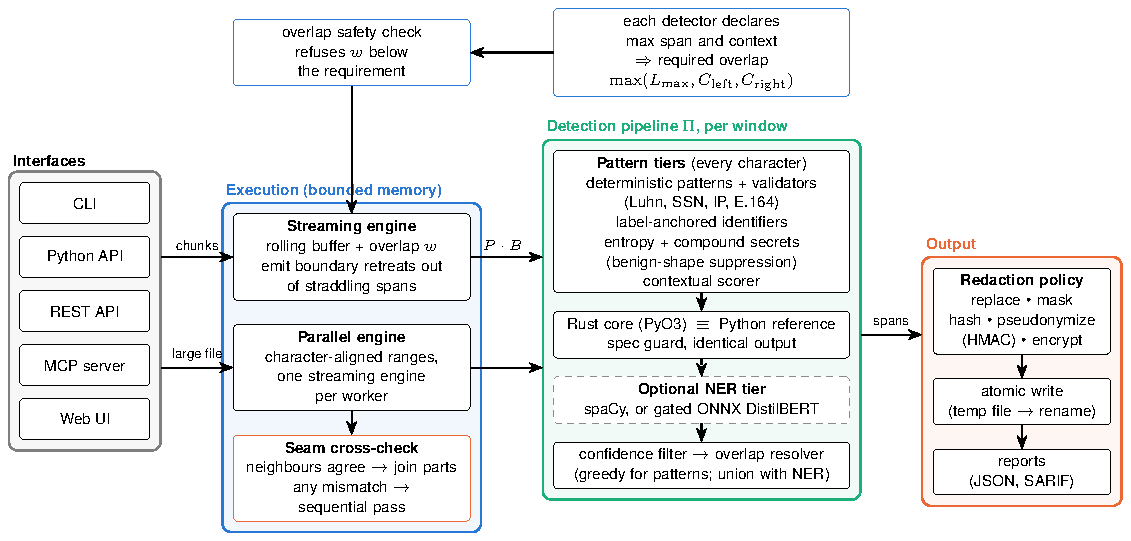
\includegraphics[width=\textwidth]{fig_architecture.pdf}
\caption{System architecture. Interfaces feed text to the streaming engine or, for a large file, to the parallel engine, whose workers each run a streaming engine and whose seams are cross-checked. Each window passes through the detection pipeline $\Pi$: the pattern tiers run on every character, on the Rust core or the identical Python reference. The dashed named-entity tier is optional; its spaCy configuration was evaluated, its ONNX configuration was not. The resolver produces disjoint spans, which the redaction policy rewrites and an atomic write commits. The overlap $w$ is checked against the maximum span and context the active detectors declare.}\label{fig:pipeline}
\end{figure*}

Figure~\ref{fig:pipeline} shows the architecture. The reference pipeline $\Pi$ runs every configured detector on a text, adjusts confidences with a bounded contextual scorer, drops detections below a threshold (0.5 by default) and resolves overlaps into a disjoint set.

\subsection{Detection tiers}

\paragraph{Deterministic patterns with validators}
Credential formats with a fixed shape (cloud access keys, provider tokens, JSON Web Tokens, PEM private-key blocks) and structured personal data (e-mail, telephone, card and social-security numbers, IPv4 and IPv6 addresses) are matched by regular expressions. A match becomes a detection only if it passes a validator: the Luhn checksum for card numbers \cite{luhn1960}, area, group and serial rules for social-security numbers, octet ranges for IPv4, address parsing for IPv6, and an E.164 shape check for telephone numbers. A generic key-assignment rule matches values that follow keys such as \texttt{api\_key}, \texttt{token} or \texttt{password}.

\paragraph{Label-anchored identifiers}
Identifiers with no checksum (patient, account or licence numbers) are ambiguous in isolation. This tier promotes a value to a detection only when a cue word that names it (for example \texttt{Patient ID:}) appears within 96 characters to its left.

\paragraph{Entropy tier with benign-shape suppression}
Candidate runs of 20 to 8192 characters over a key alphabet are scored by length, character-class mix and Shannon entropy \cite{shannon1948}, with a lower threshold for hexadecimal runs; a compound variant covers runs with embedded symbols. Entropy alone cannot separate a secret from other random-looking strings. During this study every generated UUID, commit hash, SHA-256 digest and base64 image payload in the secrets development split was flagged (Section~\ref{sec:fp}). The tier therefore suppresses three shapes: a canonical UUID, a 40- or 64-character hexadecimal value preceded by a digest cue (\texttt{commit}, \texttt{sha256}, \texttt{hash} and similar), and the payload of a \texttt{data:} URI. Suppression is vetoed when a secret-like key (\texttt{key}, \texttt{token}, \texttt{secret}, \texttt{password} and similar) names the value, so \texttt{SAUCE\_ACCESS\_KEY=}\textit{uuid} remains a secret. The check reads at most 32 characters of left context.

\paragraph{Contextual scorer}
A 48-character left window raises or lowers confidences when trigger words are present and emits a small set of trigger-gated detections of its own.

\paragraph{Optional named-entity tier}
For names, organisations and locations, an optional tier runs a spaCy pipeline (\texttt{en\_core\_web\_sm} in our experiments). An ONNX DistilBERT tier \cite{sanh2019distilbert} with a regular-expression gate in front of it is also implemented. It was \emph{not} evaluated in this study; no result in this paper comes from it, and Section~\ref{sec:neural} sets out the evaluation it requires.

\subsection{Overlap resolution}
Pattern detections that overlap are resolved best-first by confidence, then by length, so a card number beats a telephone number embedded in it. Named-entity detections are handled differently: any cluster of overlapping spans that contains a named-entity span becomes one span from the cluster's leftmost start to its rightmost end, labelled by its best pattern member if one exists. Without this union rule, a \textsc{person} tag on \texttt{john.doe} could replace the e-mail detection for \texttt{john.doe@example.com} and leave the domain exposed.

\subsection{Streaming engine}\label{sec:engine}

\begin{algorithm}[t]
\caption{Streaming detection with a bounded overlap $w$ (simplified from \texttt{engine.stream\_windows}).}\label{alg:stream}
\begin{algorithmic}[1]
\Require chunks $c_1, c_2, \dots$; detector $D$; overlap $w$; minimum emit size $m \ge w$
\State $P \gets \varepsilon$ \Comment{already emitted text, kept as read-only left context}
\State $B \gets \varepsilon$ \Comment{buffer of unemitted text}
\For{each chunk $c$}
  \State $B \gets B \cdot c$
  \If{$|B| < w + m$} \textbf{continue} \EndIf
  \State $S \gets \{(i - |P|, j - |P|, \cdot) : (i, j, \cdot) \in D(P \cdot B),\ i \ge |P|\}$ \Comment{drop spans inside $P$}
  \State $e \gets |B| - w$
  \While{some $(i, j, \cdot) \in S$ has $i < e < j$} $e \gets i$ \EndWhile \Comment{retreat out of straddlers}
  \If{$e \le 0$} \textbf{continue} \EndIf \Comment{a span pins the buffer; read more}
  \State \textbf{emit} $B[0{:}e]$ with $\{s \in S : s.j \le e\}$
  \State $P \gets \text{last } w \text{ characters of } P \cdot B[0{:}e]$; \quad $B \gets B[e{:}]$
\EndFor
\State \textbf{emit} $B$ with the spans of $D(P \cdot B)$ that start at or after $|P|$
\end{algorithmic}
\end{algorithm}

\begin{figure}[t]
\centering
\resizebox{\textwidth}{!}{%
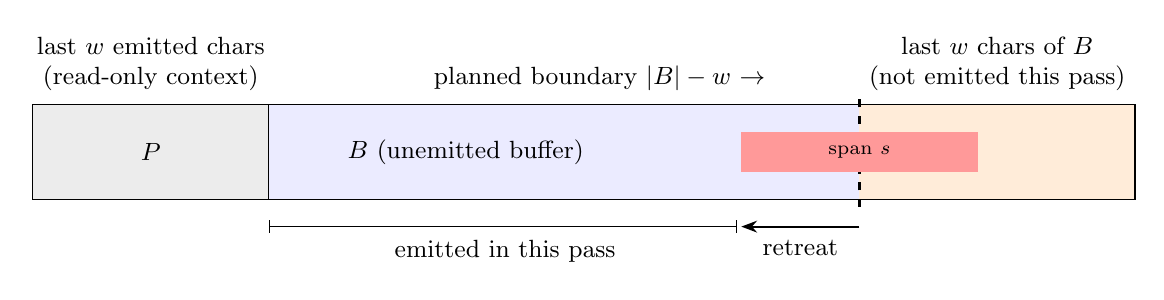
\begin{tikzpicture}[every node/.style={font=\small}]
\fill[gray!15] (0,0) rectangle (3,1.2);
\fill[blue!8] (3,0) rectangle (10.5,1.2);
\fill[orange!15] (10.5,0) rectangle (14,1.2);
\draw (0,0) rectangle (14,1.2);
\draw (3,0) -- (3,1.2);
\draw[dashed, thick] (10.5,-0.1) -- (10.5,1.3);
\node at (1.5,0.6) {$P$};
\node at (5.5,0.6) {$B$ (unemitted buffer)};
\fill[red!40] (9,0.35) rectangle (12,0.85);
\node at (10.5,0.6) {\scriptsize span $s$};
\node[above, align=center] at (1.5,1.25) {last $w$ emitted chars\\(read-only context)};
\node[above, align=center] at (12.25,1.25) {last $w$ chars of $B$\\(not emitted this pass)};
\node[above, align=center] at (7.2,1.25) {planned boundary $|B|-w$ $\rightarrow$};
\draw[-{Stealth[length=2mm]}, thick] (10.5,-0.35) -- (9,-0.35);
\node[below] at (9.75,-0.4) {retreat};
\draw[|-|] (3,-0.35) -- (8.95,-0.35);
\node[below] at (6,-0.4) {emitted in this pass};
\end{tikzpicture}}
\caption{One pass of Algorithm~\ref{alg:stream}. The detector reads $P \cdot B$; only text before the planned boundary may be emitted, and the boundary retreats out of any span that crosses it, so $s$ is carried to the next pass and detected whole.}\label{fig:window}
\end{figure}

Algorithm~\ref{alg:stream} (illustrated in Figure~\ref{fig:window}) keeps a buffer of unemitted text and the last $w$ characters already emitted. Each pass detects over their concatenation, so detectors see real left context rather than an artificial edge, and emits only the part of the buffer that lies at least $w$ characters before its end. If a detection crosses the planned emit boundary, the boundary retreats to the detection's start and the detection is carried into the next pass. Small chunks are coalesced until at least $m$ characters can be emitted, which bounds the cost of rescanning the overlap per emitted character regardless of how the input is chunked. The defaults are $w = 8192$ characters and $m = 65{,}536$ characters.

\subsection{Parallel engine}
For large files the parallel engine splits the input into character-aligned byte ranges, one per worker process. Each worker reads $w$ characters of scanned padding and a further $w$ characters of context-only prefix around its interior boundaries (seams). A span that crosses a seam belongs to the left worker, and the right worker begins emitting at that span's end. Neighbouring workers compute the seam position independently, and the coordinator compares their reports; on any disagreement it discards the parallel result and redacts the file sequentially.

\subsection{Implementation}
The pure-Python implementation is the reference. An optional Rust core implements the pattern tiers. At start-up it checks that its compiled pattern sources equal the Python ones, and it hands a window back to Python in the rare cases where Unicode case folding or floating-point summation could make the two disagree.

\paragraph{Use of AI assistance}
An AI assistant (Claude, Anthropic) was used to implement evaluation scripts and to draft this manuscript under the authors' supervision. The authors reviewed every result and every sentence and are accountable for the final content.

%% ===================================================================
\section{Formal analysis}\label{sec:formal}

Let $S_w(T)$ be the set of detections emitted by Algorithm~\ref{alg:stream} for some chunking of $T$, mapped back to absolute offsets, and $P_{w,k}(T)$ the output of the parallel engine with $k$ workers.

\begin{assumption}[Bounded span]\label{as:span}
Every detection in $\Pi(T)$ has length $j - i \le L_{\max}$.
\end{assumption}
\begin{assumption}[Bounded context]\label{as:ctx}
Whether a span $(i, j)$ belongs to $\Pi(T)$, and its final confidence, depend only on $T[i - C_{\mathrm{left}} : j + C_{\mathrm{right}}]$.
\end{assumption}

\begin{theorem}[Streaming equivalence]\label{thm:stream}
Under \ref{as:span} and \ref{as:ctx}, if
\[ w \ge \max(L_{\max}, C_{\mathrm{left}}, C_{\mathrm{right}}), \]
then $S_w(T) = \Pi(T)$ for every text $T$ and every chunking of $T$.
\end{theorem}
\begin{proof}[Proof sketch]
\emph{Completeness:} the engine emits only up to $w$ characters before the buffer's end and retreats out of any straddling span, which by \ref{as:span} is at most $L_{\max} \le w$ long; a span cut by a chunk boundary is therefore presented whole in a later pass. \emph{Soundness:} each pass detects over the last $w \ge C_{\mathrm{left}}$ emitted characters plus the buffer, and a span is emitted only if it ends at least $w \ge C_{\mathrm{right}}$ characters before the buffer's live end; both contexts are real text, so by \ref{as:ctx} every verdict and confidence equals its whole-document value. \emph{Exactly once:} a span is emitted in the unique pass whose boundary first passes its end, and emitted and carried regions are disjoint.
\end{proof}

\begin{theorem}[Parallel identity with fallback]\label{thm:par}
Under \ref{as:span} with $w \ge L_{\max}$, $P_{w,k}(T)$ equals the sequential output byte for byte. If \ref{as:span} is violated at a seam, the seam cross-check detects the disagreement and the engine falls back to sequential processing, so the outputs are equal in either case.
\end{theorem}

\begin{theorem}[Bounded working buffer]\label{thm:mem}
The working buffer of $S_w$ never exceeds $m + w + L_{\max}$ characters, independent of $|T|$; the parallel engine uses at most $k$ times that.
\end{theorem}

Because redaction is a deterministic function of $T$ and the detection set, Theorem~\ref{thm:stream} implies byte-identical redacted output. Full proofs, with each step mapped to the implementation, are in the repository's formal-model document (\url{https://github.com/MounishSenisetty/SafeStream-Redactor/blob/0765dae/docs/FORMAL_MODEL.md}); the sketches above are not a substitute for them and were not machine-checked.

\paragraph{What is derived and what is assumed}
Each detector declares its maximum span and the left and right context it reads, and the engine sizes its overlap from the maximum over active detectors and refuses to start with less unless the caller explicitly overrides it. For the default pipeline the declarations give $C_{\mathrm{left}} = 96$ (the label-anchored cue window), $C_{\mathrm{right}} = 8$ and $L_{\max} = 8192$ (bounds on private-key blocks and entropy candidates), so the default $w = 8192$ satisfies Theorem~\ref{thm:stream}. A regression test fails if any declaration changes these values, and a differential test probes each detector to check that its real context dependency does not exceed its declaration. Two parts of \ref{as:span} and \ref{as:ctx} are \emph{not} derived from declarations and should be read as assumptions corroborated by tests rather than proven properties of the code: (i) the confidence adjustment and threshold must not reach beyond the declared context, and (ii) overlap resolution must not propagate decisions along chains of overlapping candidates further than $C_{\mathrm{left}}$ or $C_{\mathrm{right}}$, and the named-entity union rule must not create spans longer than $L_{\max}$. For the pattern tiers, whose spans are bounded and whose overlaps are short, the equivalence tests in Section~\ref{sec:equiv} found no counterexample; for a statistical model, whose output can depend on its whole input window, the declared bounds (256 characters for the spaCy tier) are declarations only, and the theorems should not be read as covering it.

\paragraph{Failure modes}
Lowering the overlap below the declared requirement is refused by default; if a caller overrides that, the parallel engine still falls back safely, but the sequential engine can split a long span. A detector that understates its context, or one that needs document-wide context, is outside the guarantee.

%% ===================================================================
\section{Experimental methodology}\label{sec:setup}

The evaluation addresses five questions. \textbf{RQ1}: do the implementation's streamed, parallel and native outputs match the reference in practice? \textbf{RQ2}: how do memory and throughput scale? \textbf{RQ3}: how well do the pattern tiers detect credentials compared with purpose-built scanners? \textbf{RQ4}: how well does SafeStream detect personal data compared with Presidio, with and without a named-entity model? \textbf{RQ5}: how much protection does it give at the level of a whole document, and how much of that depends on rules written after seeing the benchmark?

\subsection{Corpora and splits}
Table~\ref{tab:corpora} lists the test splits. Each corpus was split once into development and test halves with a fixed seed. The manifests list document identifiers and the SHA-256 of the source data, and the loader refuses a source that no longer matches. Development, error analysis and tuning used development halves only, with the exception of RedactionBench described below; test halves were scored after the code was frozen, with one disclosed exception (Section~\ref{sec:fp}).
\begin{itemize}
\item \textbf{presidio-research} \cite{presidioresearch} (synthetic): the dataset distributed with Presidio's evaluation toolkit (revision 0cb3650), with person, location, organisation, telephone, card, date and other labels, generated from templates.
\item \textbf{secrets} (semi-synthetic): the labelled examples in the Nosey Parker rule set \cite{noseyparker} (revision 2e6e7f3) as positives, with gold spans given by each rule's own capture groups, plus 200 generated non-secrets (UUIDs, commit hashes, SHA-256 digests, base64 image payloads, minified JavaScript) as gold-free documents. The split is by rule, so the test half contains vendor formats absent from the development half. The positives are short examples written by rule authors, not credentials observed in real artefacts.
\item \textbf{RedactionBench} \cite{brynjolfsson2026redactionbench}: 200 documents across eleven domains, a majority seeded from real-world sources according to its authors, with character spans labelled \emph{mandatory} or \emph{contextual}. All 200 documents were used for error analysis and rule writing before the split existed, so its test half is not held out (Section~\ref{sec:contam}).
\end{itemize}

\begin{table}[t]
\centering
\caption{Test splits. Gold-free documents contain no gold span; any detection on them is a false alarm.}\label{tab:corpora}
\resizebox{\textwidth}{!}{%
\begin{tabular}{lrrrr}
\toprule
Corpus & Documents & Gold spans & Gold-free docs & Size (bytes) \\
\midrule
presidio-research & 750 & 1,394 & 63 & 63,678 \\
secrets & 313 & 293 & 97 & 46,595 \\
RedactionBench & 100 & 25,592 & 0 & 1,378,267 \\
\bottomrule
\end{tabular}}
\end{table}

\subsection{Systems and configurations}
\textbf{SafeStream} was run with the Rust core and default tiers (\emph{pattern}), with the opt-in date tier (\emph{+dates}), and with the spaCy \texttt{en\_core\_web\_sm} tier (\emph{+spaCy}). \textbf{Presidio} 2.2.355 \cite{presidio} was run as its pattern recognisers alone (\emph{regex}) and as the full analyser with spaCy \texttt{en\_core\_web\_sm} (\emph{sm}) and \texttt{en\_core\_web\_lg} (\emph{lg}), with spaCy 3.8.13 and models 3.8.0. \textbf{gitleaks} 8.28.0 \cite{gitleaks} and \textbf{TruffleHog} 3.90.8 \cite{trufflehog} were run with default rules and default false-positive filtering; TruffleHog ran with \texttt{--no-verification}, so no example credential was sent to a live service. Each scanner ran once over a directory with one file per document, and findings were mapped back to character offsets; TruffleHog's composite findings (for example \texttt{user:token}) were credited for each component that appears in the text. Each Python tool ran in its own virtual environment and process, pinned to one thread; the scanners are Go binaries and ran with their default concurrency. All SafeStream thresholds are defaults; no threshold was tuned on test data. The RedactionBench dev-selected configurations (Section~\ref{sec:contam}) were chosen on the development half by a rule fixed in advance.

\subsection{Metrics}
Let $G$ and $R$ be the sets of gold and redacted character positions in a document. Character precision and recall are $|G \cap R| / |R|$ and $|G \cap R| / |G|$, summed over documents, and F1 is their harmonic mean. All metrics are type-agnostic: a value counts as protected whatever label it receives. The \emph{fully redacted rate} is the share of gold spans with every character redacted. The \emph{false-alarm document rate} is the share of gold-free documents with at least one detection. On RedactionBench, \emph{mandatory recall} is character recall over mandatory spans, and the \emph{no-leak document rate} is the share of documents in which every mandatory character is redacted (Section~\ref{sec:noleak} discusses how it relates to recall).

\subsection{Statistical analysis}
We report 95\% percentile bootstrap intervals over documents (2,000 resamples). Differences between two systems are computed on the same resamples (paired bootstrap), and a difference is called significant only when its paired interval excludes zero; where we compare intervals that were not computed jointly, we say so and do not treat non-overlap as a test. Three caveats apply. First, documents are not independent: secrets positives cluster by rule (several examples per rule) and presidio-research documents are generated from shared templates, so document-level intervals are likely too narrow; a cluster bootstrap by rule or template was not performed. Second, no correction for multiple comparisons was applied; the comparisons in the abstract were planned, the ablation comparisons were not. Third, the analysis was not pre-registered.

\subsection{Environment}
Accuracy runs used a 4-vCPU Intel Xeon virtual machine at 2.80\,GHz with 15\,GB RAM, Linux and CPython 3.13.16. Throughput figures come from separate runs, five per configuration, on the same machine with no other benchmark running; the throughput recorded during accuracy runs is not used. Memory was measured as the peak resident set size of a fresh process per point minus its resident set size after imports, so native allocations are included; it is reported in MiB.

%% ===================================================================
\section{Results}\label{sec:results}

\subsection{RQ1: equivalence and backend parity}\label{sec:equiv}
On every test split the Rust core and the pure-Python reference produced identical predictions (presidio-research 178 spans, secrets 298, RedactionBench 3,167, from the frozen commit). The repository's equivalence suite asserts byte-identical streamed, whole-document and parallel output over exhaustive small chunkings, property-based generated inputs, seam-straddling entities and forced fallbacks, and also checks native parity and declared context; it passed 133 of 133 tests at the final commit. These tests corroborate the theorems for the configurations they exercise; they are not proofs, and they do not exercise the named-entity tier's full input dependence.

\subsection{RQ2: memory and throughput}\label{sec:memory}

\begin{figure}[t]
\centering
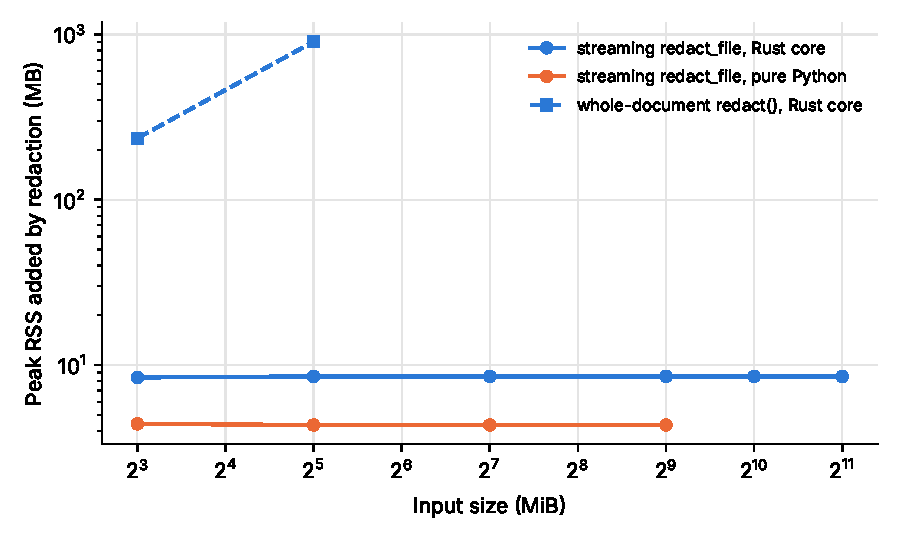
\includegraphics[width=0.85\textwidth]{fig_memory.pdf}
\caption{Peak resident memory added by redaction (peak RSS minus RSS after imports, MiB) against input size, log scales, each point a fresh process. Streaming \texttt{redact\_file} stays flat from 8\,MiB to 2\,GiB (Rust core) and to 512\,MiB (pure Python); whole-document \texttt{redact()} grows with the input.}\label{fig:memory}
\end{figure}

Figure~\ref{fig:memory} plots peak resident memory against input size. Each point is a fresh process redacting a generated log file dense with personal data and credentials. With the Rust core, streaming \texttt{redact\_file} added between 8.4 and 8.54\,MiB at every size from 8\,MiB to 2\,GiB, a 256-fold range. The pure-Python backend added between 4.3 and 4.4\,MiB from 8 to 512\,MiB; it was not run at larger sizes because of its run time (726\,s at 512\,MiB). Whole-document \texttt{redact()} on the same generated inputs, measured the same way, added 235.5\,MiB at 8\,MiB and 904.6\,MiB at 32\,MiB, about 28 times the input size, because the input string, the detections and the output are held at once; at 32\,MiB the two modes therefore differ by a factor of about 106 on identical input. A 128\,MiB whole-document run was stopped after 20 minutes without completing and is not reported. These measurements are consistent with Theorem~\ref{thm:mem} but cover one generated input shape on one machine, and only two whole-document sizes.

\begin{table}[t]
\centering
\small
\caption{Throughput on the test splits in MB/s, mean $\pm$ sample standard deviation over 5 runs, one thread, load time excluded. Each run is a fresh process on an otherwise idle 4-vCPU machine.}\label{tab:throughput}
\resizebox{\textwidth}{!}{%
\begin{tabular}{llll}
\toprule
System & presidio-research & secrets & RedactionBench \\
\midrule
SafeStream pattern (Rust core) & 1.82 $\pm$ 0.42 & 2.39 $\pm$ 0.58 & 10.4 $\pm$ 1.3 \\
SafeStream pattern (pure Python) & 1.1 $\pm$ 0.07 & 0.916 $\pm$ 0.17 & 1.23 $\pm$ 0.15 \\
SafeStream +spaCy (sm) & 0.0118 $\pm$ 0.0009 & 0.0227 $\pm$ 0.0034 & 0.0467 $\pm$ 0.0033 \\
Presidio regex & 0.0802 $\pm$ 0.0127 & 0.0983 $\pm$ 0.0155 & 0.0694 $\pm$ 0.0028 \\
Presidio sm & 0.0081 $\pm$ 0.0004 & 0.0125 $\pm$ 0.0007 & 0.0201 $\pm$ 0.0003 \\
Presidio lg & 0.0074 $\pm$ 0.0010 & 0.0128 $\pm$ 0.0008 & 0.0203 $\pm$ 0.0003 \\
gitleaks$^{a}$ & 0.507 $\pm$ 0.028 & 0.409 $\pm$ 0.051 & 3.15 $\pm$ 0.19 \\
TruffleHog$^{a}$ & 0.0269 $\pm$ 0.0016 & 0.0188 $\pm$ 0.0007 & 0.594 $\pm$ 0.02 \\
\bottomrule
\end{tabular}}

\smallskip
\footnotesize $^{a}$ Go binaries run once per corpus over a directory of documents; the figure includes process start-up and is not limited to one thread.
\end{table}

Table~\ref{tab:throughput} reports throughput on the test splits. Per-document overhead dominates on presidio-research and secrets, whose documents average 85 and 149 bytes; RedactionBench's documents average 13.8\,kB. There the Rust core processed 10.4 $\pm$ 1.3\,MB/s, the pure-Python reference 1.23 $\pm$ 0.15\,MB/s and Presidio's pattern recognisers 0.069\,MB/s. With a statistical model in the loop every system ran below 0.05\,MB/s: SafeStream +spaCy at 0.047\,MB/s and Presidio sm and lg at 0.020\,MB/s. The scanner figures include process start-up and are not comparable per thread.

\begin{figure}[t]
\centering
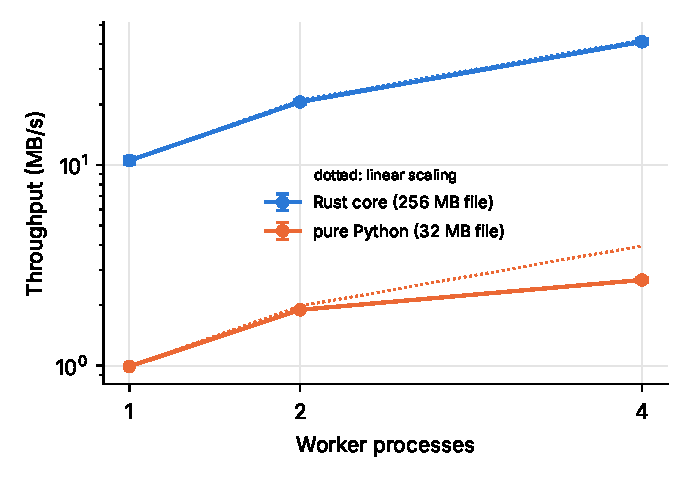
\includegraphics[width=0.62\textwidth]{fig_scaling.pdf}
\caption{Throughput of \texttt{redact\_file} against worker processes on a 4-vCPU machine, mean and standard deviation over 5 runs (log scale). Dotted lines show linear scaling from one worker. The parallel output is byte-identical to the sequential output (Theorem~\ref{thm:par}).}\label{fig:scaling}
\end{figure}

On a single 256\,MB generated log file (mostly benign log lines and prose with personal data and credentials mixed in), \texttt{redact\_file} with the Rust core ran at 10.5 $\pm$ 0.5, 20.6 $\pm$ 0.5 and 41.1 $\pm$ 1.4\,MB/s with 1, 2 and 4 worker processes, a 3.9-fold speed-up on 4 vCPUs (Figure~\ref{fig:scaling}). The pure-Python backend on a 32\,MB file of the same kind ran at 0.99, 1.90 and 2.67\,MB/s. These figures come from one virtual machine and should be read as relative rather than absolute.

\subsection{RQ3 and RQ4: detection on held-out data}

\begin{figure}[t]
\centering
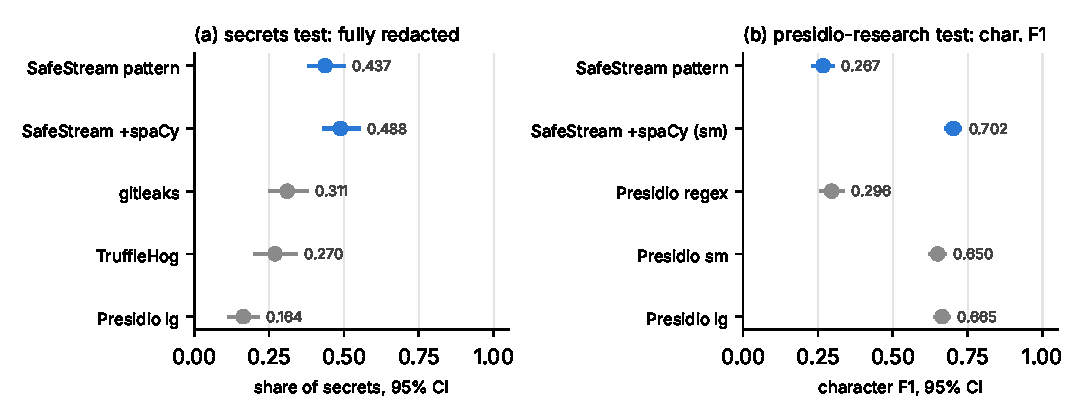
\includegraphics[width=\textwidth]{fig_accuracy.pdf}
\caption{Test-split accuracy with 95\% bootstrap intervals. (a) Share of secrets fully redacted on the secrets test split. (b) Character F1 on the presidio-research test split. SafeStream configurations in blue, baselines in grey.}\label{fig:accuracy}
\end{figure}

\begin{table}[t]
\centering
\small
\caption{Test-split results with 95\% bootstrap intervals. SafeStream rows are after the entropy fix of Section~\ref{sec:fp}, which changed only the secrets results. FR: fully redacted rate; FA: false-alarm document rate.}\label{tab:main}
\resizebox{\textwidth}{!}{%
\begin{tabular}{llllll}
\toprule
Corpus / system & Char P & Char R & Char F1 & FR & FA \\
\midrule
\multicolumn{6}{l}{\emph{presidio-research (750 documents)}}\\
SafeStream pattern & .995 [.992,.998] & .154 [.133,.176] & .267 [.235,.299] & .115 [.098,.134] & .000 \\
SafeStream +dates & .996 [.993,.998] & .169 [.146,.192] & .290 [.255,.322] & .129 [.110,.150] & .000 \\
SafeStream +spaCy (sm) & .898 [.877,.918] & .576 [.547,.606] & .702 [.679,.725] & .538 [.509,.568] & .079 \\
Presidio regex & .948 [.919,.974] & .175 [.151,.202] & .296 [.260,.333] & .123 [.105,.145] & .000 \\
Presidio sm & .871 [.848,.893] & .518 [.491,.546] & .650 [.626,.673] & .506 [.479,.536] & .048 \\
Presidio lg & .878 [.856,.900] & .535 [.507,.563] & .665 [.642,.688] & .562 [.534,.590] & .000 \\
\midrule
\multicolumn{6}{l}{\emph{secrets (313 documents)}}\\
SafeStream pattern & .857 [.705,.946] & .829 [.740,.887] & .842 [.736,.906] & .437 [.384,.498] & .010 \\
SafeStream +spaCy (sm) & .757 [.604,.858] & .845 [.762,.897] & .799 [.683,.870] & .488 [.435,.548] & .340 \\
gitleaks & .837 [.630,.962] & .473 [.299,.679] & .604 [.430,.765] & .311 [.253,.375] & .000 \\
TruffleHog & .803 [.719,.878] & .189 [.117,.308] & .306 [.204,.446] & .270 [.204,.340] & .000 \\
Presidio regex & .282 [.211,.356] & .105 [.063,.177] & .153 [.098,.225] & .126 [.083,.168] & .392 \\
Presidio sm & .251 [.191,.315] & .119 [.072,.197] & .161 [.107,.232] & .160 [.112,.206] & .649 \\
Presidio lg & .308 [.238,.381] & .131 [.082,.214] & .184 [.124,.262] & .164 [.116,.212] & .433 \\
\bottomrule
\end{tabular}}
\end{table}

Table~\ref{tab:main} and Figure~\ref{fig:accuracy} give the test-split results.

\paragraph{Credentials (RQ3)}
On secrets, SafeStream's pattern tiers fully redacted 0.437 of test secrets, against 0.311 for gitleaks and 0.270 for TruffleHog. The paired differences in fully redacted rate were $+0.128$ [$+0.073$, $+0.183$] and $+0.167$ [$+0.079$, $+0.250$], and in character F1 $+0.233$ [$+0.043$, $+0.441$] and $+0.536$ [$+0.310$, $+0.685$]. The differences in character precision were not significant ($+0.005$ [$-0.063$, $+0.123$] and $+0.060$ [$-0.109$, $+0.176$]). SafeStream flagged one of 97 generated non-secrets; neither scanner flagged any. More than half of the test secrets (0.563) were not fully redacted by SafeStream either. The development recall (0.542) exceeded the test recall (0.437) because the test half holds vendor formats for which SafeStream has no pattern. Presidio has no credential recognisers, and adding spaCy raised SafeStream's false-alarm rate to 0.340; on the development split those false alarms were the word \texttt{Merge} in commit lines tagged as a person and digest or UUID tokens tagged as persons or organisations.

This comparison has a fairness caveat that we could not resolve with the available runs. The gold labels are Nosey Parker's rule examples, and both scanners apply false-positive filters (allowlists of placeholder-like values in gitleaks, result filtering in TruffleHog) designed to suppress example-like strings. Default configurations reflect how the tools are used, but the corpus may penalise these filters more than real data would. A sensitivity run with the filters disabled was not performed (Section~\ref{sec:plan}). SafeStream's own credential patterns were not developed on this corpus: it was added after the split was fixed, and the only change made using it was the suppression rule of Section~\ref{sec:fp}, designed on the development half.

\paragraph{Personal data (RQ4)}
On presidio-research, the pattern tiers were precise (character precision 0.995) but recalled only 0.154 of sensitive characters, because most gold spans are names, locations and organisations that patterns cannot capture. Against Presidio's pattern recognisers, the paired difference in character recall was $-0.021$ [$-0.041$, $-0.002$] and in precision $+0.047$ [$+0.021$, $+0.076$]. With the same spaCy model, SafeStream +spaCy exceeded Presidio sm in character F1 by $+0.051$ [$+0.027$, $+0.076$] and in fully redacted rate by $+0.031$ [$+0.004$, $+0.060$]. Against Presidio lg, which uses a larger model, SafeStream +spaCy had higher character F1 ($+0.036$ [$+0.011$, $+0.064$]), but the difference in fully redacted rate, $-0.025$ [$-0.053$, $+0.004$], was not significant. This corpus is synthetic and template-generated; the comparison shows relative behaviour on that distribution only.

\subsection{False alarms on high-entropy non-secrets}\label{sec:fp}

Before the fix described in Section~\ref{sec:method}, SafeStream flagged 83 of the 103 generated non-secrets in the development split (false-alarm rate 0.806), all through the entropy tier: every UUID, commit hash, SHA-256 digest and base64 image payload, and none of the minified JavaScript. The suppression rule was designed on the development split. A first version cost one development secret, a UUID-shaped access key assigned to \texttt{SAUCE\_ACCESS\_KEY}, which led to the secret-key veto. With the veto, the development false-alarm rate fell to 0.000 with no change in recall, and the presidio-research and RedactionBench development results were unchanged except in the fourth decimal. On the test split, the false-alarm rate fell from 0.794 [0.714, 0.872] to 0.010 [0.000, 0.035], character precision rose from 0.589 to 0.857, and recall was unchanged (0.829 character recall, 0.437 fully redacted). The test half had been scored once with the pre-fix code before the fix was made; both scores are reported. Because the gold-free documents in both halves come from the same generator, the test improvement is an optimistic estimate of the fix's effect on real non-secrets.

\subsection{RQ5: document-level protection and contamination}\label{sec:contam}

\begin{table}[t]
\centering
\small
\caption{RedactionBench test half (100 documents). \emph{Exposed}: current code, whose rules were written after inspecting all 200 documents. \emph{Pre-exposure}: the last commit before the benchmark entered the repository. \emph{Dev-selected}: configuration chosen on the development half by a fixed rule (maximum development character F1) and scored on the test half once.}\label{tab:rb}
\resizebox{\textwidth}{!}{%
\begin{tabular}{llll}
\toprule
System & Char F1 & Mandatory recall & No-leak docs \\
\midrule
Pre-exposure, pattern & .518 [.434,.593] & .589 [.476,.696] & .074 [.022,.129] \\
Pre-exposure, +spaCy & .472 [.395,.547] & .674 [.566,.779] & .137 [.073,.208] \\
Pre-exposure, dev-selected & .469 [.394,.543] & .676 [.568,.781] & .137 [.073,.208] \\
Exposed, pattern & .579 [.490,.662] & .682 [.578,.787] & .084 [.032,.144] \\
Exposed, +spaCy & .512 [.429,.590] & .761 [.657,.860] & .179 [.105,.263] \\
Exposed, dev-selected & .508 [.427,.588] & .762 [.658,.862] & .179 [.105,.263] \\
\midrule
gitleaks & .214 [.130,.314] & .247 [.140,.372] & .021 [.000,.053] \\
TruffleHog & .030 [.017,.048] & .024 [.013,.040] & .000 \\
Presidio regex & .323 [.250,.393] & .331 [.227,.422] & .011 [.000,.033] \\
Presidio sm & .336 [.265,.402] & .416 [.326,.500] & .084 [.032,.146] \\
Presidio lg & .344 [.277,.409] & .420 [.333,.499] & .105 [.052,.174] \\
\bottomrule
\end{tabular}}
\end{table}

Table~\ref{tab:rb} separates the contaminated and uncontaminated results. Rules written after inspecting the benchmark raised test mandatory recall of the pattern tiers by $+0.091$ [$+0.044$, $+0.163$] and character F1 by $+0.060$ [$+0.029$, $+0.108$] relative to the pre-exposure code (paired). Because those rules were written while the test documents were visible, this gain is an upper bound on what they contribute to unseen data. One of them, the label-anchored tier, also improved presidio-research, a corpus it was never tuned on (Table~\ref{tab:ablation}), which is evidence that it generalises. Development-set selection chose the same configuration for both code versions (spaCy on, entropy on, confidence threshold 0.3). The pre-exposure code, which never saw the benchmark, had higher mandatory recall with spaCy (0.674 [0.566, 0.779]) and higher pattern-tier character F1 (0.518 [0.434, 0.593]) than any Presidio configuration (at most 0.420 [0.333, 0.499] and 0.344 [0.277, 0.409]); these intervals were not computed jointly, so the comparison is descriptive rather than a paired test.

\paragraph{No-leak documents}\label{sec:noleak}
The no-leak document rate was low for every system: at most 0.179 [0.105, 0.263] for SafeStream (+spaCy, exposed code), 0.137 for the pre-exposure code with spaCy, 0.084 for the pattern tiers alone, and at most 0.105 for Presidio. In other words, for at least 82\% of RedactionBench test documents, every configuration we evaluated left at least one must-redact character in the clear. This metric is deliberately strict. Mandatory recall measures the share of must-redact characters hidden; the no-leak rate requires all of them in a document to be hidden, so a single missed character fails the document. RedactionBench documents are dense: the test half averages about 256 gold spans per document (Table~\ref{tab:corpora}), of which 84 on average (median 25) are mandatory. As an illustration only, if a document had $n$ independent must-redact units each detected with probability $p$, it would be leak-free with probability $p^{n}$, which for $n$ in the hundreds is small even for $p$ close to one; real misses are correlated (whole entity types missing in a domain), so this is not a model of the data, but it shows why per-character recall in the 0.68--0.76 range is compatible with almost no fully protected documents. 

\emph{Where the leaks are.} We re-ran five systems of Table~\ref{tab:rb} (exposed pattern tiers, exposed +spaCy, gitleaks, TruffleHog and Presidio lg) on the test half at the commit that produced those rows, reproducing its mandatory recall and no-leak rates exactly, and kept the per-document predictions (script \texttt{benchmarks/leak\_analysis.py}; aggregates in \texttt{2026-10-11\_redactionbench\_test\_leak\_analysis.json}). The 95 test documents with mandatory gold contain 8{,}002 mandatory spans. Three observations follow; they are descriptive, from one corpus that had been inspected during development, and carry no confidence intervals.
\begin{itemize}
\item \emph{Leaks are whole misses, not boundary errors.} With spaCy, 6{,}441 mandatory spans were fully redacted, 64 partially and 1{,}497 not at all; of the 17{,}122 leaked mandatory characters, 826 (4.8\%) lie in partially redacted spans and the rest in spans with no detection. For the pattern tiers alone the share is 3.7\% (854 of 22{,}778). Presidio lg leaks more through partial coverage: 7{,}354 of its 41{,}589 leaked characters (17.7\%).
\item \emph{Few documents are near misses; leaks are concentrated.} With spaCy, 17 documents leaked nothing, 5 more leaked exactly one mandatory span and 7 more leaked two, so fixing one or two spans per document would raise the no-leak rate to at most 29 of 95 (0.305). The median document leaked 6 mandatory spans (interquartile range 2--16), a median of 23\% of its mandatory spans, and the 9 documents with the most leaked characters held 67\% of them. For the pattern tiers alone the median document leaked 11 spans (52\%), and only 2 documents were within two spans of no leak.
\item \emph{What is missed.} The corpus carries no entity types, so we grouped spans by a coarse shape heuristic. Capitalised words (largely names) leaked at a rate of 0.90 without a named-entity model and 0.27 with spaCy, which accounts for most of the gap between the two configurations. Spans containing \texttt{@} leaked at 0.95 (36 of 38) with spaCy; inspection of a few of them, after all scores were final, showed passwords inside connection strings or quoted configuration values that the e-mail pattern split or that no tier matched. No code was changed in response, and these spans should not be read as a test-set error analysis used for tuning.
\end{itemize}
Even an oracle that took the union of all five systems' redactions would leave 69 of 95 documents leaking (no-leak rate 0.274), so the low document-level rate is a property of the corpus and of current detectors in general, not only of SafeStream. The low rate is not caused by streaming: by Theorem~\ref{thm:stream} the streamed output equals the whole-document output, so these leaks are detection misses that a whole-document run would also make.

\subsection{Ablation}

\begin{table}[t]
\centering
\small
\caption{Ablation on the test splits (pure-Python backend, identical output to the Rust core). Paired differences against the full pattern pipeline, with 95\% intervals; FR: fully redacted rate.}\label{tab:ablation}
\resizebox{\textwidth}{!}{%
\begin{tabular}{llll}
\toprule
Change & secrets & presidio-research & RedactionBench \\
\midrule
\multicolumn{4}{l}{\emph{Character F1, full pattern pipeline minus variant}}\\
Remove entropy tier & $+.455$ [.242,.641] & $.000$ & $+.156$ [.104,.224] \\
Remove label-anchored tier & $.000$ & $+.030$ [.019,.044] & $+.004$ [.002,.006] \\
Remove contextual detections & $.000$ & $.000$ & $.000$ \\
\midrule
\multicolumn{4}{l}{\emph{Union rule versus greedy resolution (with spaCy), union minus greedy}}\\
Character recall & $+.006$ [.000,.017] & $+.005$ [.002,.008] & $+.009$ [.004,.016] \\
FR / mandatory recall$^{a}$ & $+.013$ [.000,.032] & $+.001$ [.000,.002] & $+.012$ [.004,.022] \\
\bottomrule
\end{tabular}}

\smallskip
\footnotesize $^{a}$ Fully redacted rate for secrets and presidio-research; mandatory recall for RedactionBench.
\end{table}

Table~\ref{tab:ablation} isolates the components. The entropy tier carried most of the credential recall: without it, character F1 on secrets fell from 0.842 to 0.383. The label-anchored tier mattered on presidio-research, where several identifiers carry labels. The contextual scorer's own detections changed no result on these corpora; its confidence adjustment was kept in every variant. Alone, the deterministic tier reached a character F1 of 0.380 on secrets and 0.237 on presidio-research, and the entropy tier alone 0.822 on secrets. The union rule raised recall by small and mostly significant amounts at no significant cost in F1 on secrets ($+0.000$ [$-0.003$, $+0.005$]) and RedactionBench ($+0.003$ [$-0.002$, $+0.008$]); on presidio-research its F1 difference was $+0.004$ [$+0.001$, $+0.007$]. The effect of the gate in front of the ONNX tier was not measured.

%% ===================================================================
\section{Discussion}\label{sec:discussion}

\subsection{What the results establish, and what they do not}
\emph{Established under stated assumptions:} chunked and parallel processing introduce no detection difference relative to the whole-document pipeline, for detectors that respect their declared bounds (Section~\ref{sec:formal}). \emph{Measured:} flat working memory across a 256-fold range of input sizes on one input shape; near-linear scaling to four cores; on held-out splits, higher credential coverage than two scanners in default configurations on a corpus of rule examples, and higher F1 than Presidio with the same spaCy model on a synthetic corpus. \emph{Not established:} effectiveness on real-world artefacts; document-level protection adequate for public release; any property of the ONNX tier; robustness to adversarial obfuscation.

\subsection{When is the approach useful despite a low no-leak rate?}
Bounded memory and equivalence do not make redaction complete; they remove one specific failure mode, the leak introduced by chunking itself, and make large inputs processable at all. The value of that depends on the detection coverage for the values that matter in a given deployment. The evidence supports three uses and argues against a fourth.
\begin{enumerate}
\item \emph{Defence in depth for structured secrets in machine-generated text.} Where the sensitive values are credentials and structured identifiers with recognisable shapes (logs, configuration dumps, CI output), the pattern tiers are where coverage is highest in our data, and the guarantee ensures that splitting a multi-gigabyte log does not make coverage worse. Even here more than half of the test secrets were not fully redacted, so the tool reduces exposure rather than eliminating it.
\item \emph{Pre-filtering before human review or controlled sharing.} When output is reviewed, or shared only with parties already bound by agreements, a high-precision filter that reliably processes large inputs reduces the volume of exposed values without being the last line of defence.
\item \emph{Inputs that cannot otherwise be processed.} Whole-document redaction needed about 28 times the input size in memory in our measurements, which rules it out for multi-gigabyte files on ordinary hosts.
\item \emph{Not supported: sole control for public release of free text.} With no-leak rates below 0.18 on RedactionBench and low free-text recall without a named-entity model, the results do not justify releasing redacted free-text documents publicly on the strength of this system alone.
\end{enumerate}
A deployment should set its own acceptance criteria before relying on the system, for example: per-category recall measured on a representative, authorised sample of the target artefacts; zero tolerated leaks for specified credential types on that sample; a review step for document classes with free text; and periodic re-measurement as formats change. None of these was measured here.

\subsection{Threats to validity}
\emph{External validity.} presidio-research is synthetic and template-generated; the secrets positives are rule-author examples and the negatives are generated from five templates; RedactionBench is the only corpus with real-world seeding, and it is contaminated. The corpora are English-only. No result here establishes performance on real logs or exports. \emph{Construct validity.} The secrets gold spans are Nosey Parker's capture groups, so credentials adjacent to a labelled secret (for example a client identifier next to its secret) count as false positives; RedactionBench's contextual labels have low human agreement according to its authors \cite{brynjolfsson2026redactionbench}. \emph{Internal validity.} The secrets test half was scored before and after one fix (Section~\ref{sec:fp}); RedactionBench was inspected during development. \emph{Statistical validity.} Bootstrap intervals assume independent documents, which overstates precision for clustered corpora, and no multiplicity correction was applied. \emph{Comparison fairness.} The scanners were run with default filters on a corpus of examples those filters target. \emph{Environment.} All runs used one virtual machine.

\subsection{The unevaluated neural tier}\label{sec:neural}
The ONNX tier and its gate are implemented but contribute no result in this paper; its models and the corpora for evaluating it are hosted on a service the evaluation environment could not reach. Evaluating it requires: (i) data: the ai4privacy test split \cite{ai4privacy300k} under its licence and the Text Anonymization Benchmark \cite{pilan2022tab}, excluding CoNLL-2003 from claims because the bundled model was trained on it \cite{tjongkimsang2003conll}; (ii) baselines: Presidio with transformer models and a generalist span model \cite{zaratiana2024gliner}; (iii) metrics: the same character, fully-redacted and no-leak metrics, plus throughput and peak memory; (iv) an ablation of the gate (fraction of characters reaching the model and recall lost); (v) an empirical equivalence check, comparing streamed and whole-document output with the model enabled, because the theorems do not cover a model whose output depends on its whole input window; (vi) pinned model files, hashes and split manifests.

\subsection{Evaluation plan for real-world evidence}\label{sec:plan}
Ranked by expected value per unit of effort:
\begin{enumerate}
\item \emph{Cluster bootstrap} by rule (secrets) and by template where identifiable (presidio-research), to correct intervals for dependence.
\item \emph{Scanner sensitivity analysis:} gitleaks and TruffleHog with their false-positive filters disabled, reported alongside the defaults.
\item \emph{Real credential-bearing text with clear provenance:} public CI logs or issue attachments from repositories whose licences permit research use, or logs from an organisation that authorises the study. Safeguards: never test discovered credentials against live services; store raw text encrypted with access limited to annotators; report discovered live secrets to their owners through responsible disclosure; publish only annotations, hashes and aggregate results, not secret values; obtain ethics review where required; double annotation with agreement reported.
\item \emph{The neural-tier evaluation} of Section~\ref{sec:neural}.
\item \emph{A second machine} for throughput and memory, to separate implementation effects from the virtual machine.
\end{enumerate}

%% ===================================================================
\section{Conclusion}\label{sec:conclusion}
Chunked redaction need not trade correctness for scale. With detector-declared bounds on span length and context, a bounded overlap makes the streamed result equal to the whole-document result, a seam cross-check makes the parallel result equal to the sequential one, and the working buffer does not grow with the input; in our measurements memory stayed flat from 8\,MiB to 2\,GiB and throughput scaled 3.9-fold on four cores. These properties remove chunking as a source of leaks; they do not make detection complete. On held-out data, the pattern tiers covered more credentials than gitleaks and TruffleHog in default configurations, and with a spaCy model SafeStream was more accurate than Presidio with the same model on a synthetic corpus, but fewer than one RedactionBench document in five was fully protected by any configuration and two of the three corpora are synthetic. The system is therefore suited to reducing exposure in large machine-generated artefacts as one layer among several, not to certifying documents for public release. The next steps are evaluation on authorised real-world text, the neural tier, and the statistical refinements listed in Section~\ref{sec:plan}.

%% ===================================================================
\section*{CRediT authorship contribution statement}
\MISSING{each author's CRediT roles (Conceptualization, Software, Validation, Formal analysis, Investigation, Writing -- original draft, Writing -- review \& editing, Supervision)}

\section*{Declaration of competing interest}
\MISSING{The authors declare that they have no known competing financial interests or personal relationships that could have appeared to influence the work reported in this paper. -- confirm or replace}

\section*{Funding}
\MISSING{funding sources, or: This research did not receive any specific grant from funding agencies in the public, commercial, or not-for-profit sectors.}

\section*{Ethics statement}
No human participants were involved. All corpora are public or generated. The secrets corpus consists of example strings published in an open-source rule set; no credential was tested against a live service (TruffleHog ran without verification). The ai4privacy corpus was not used.

\section*{Data availability}
Source code, split manifests, the evaluation harness and raw results are available at \url{https://github.com/MounishSenisetty/SafeStream-Redactor}; every number in this article is generated from files under \texttt{research/results/}. \MISSING{archive a tagged release (e.g.\ on Zenodo) and give its DOI here}. presidio-research and Nosey Parker are public; RedactionBench is available from its authors under CC BY 4.0. Generated non-secrets are produced by the released code with a fixed seed.

\section*{Declaration of generative AI and AI-assisted technologies in the writing process}
During the preparation of this work the authors used Claude (Anthropic) to implement evaluation scripts and to draft the manuscript text. After using this tool, the authors reviewed and edited the content as needed and take full responsibility for the content of the publication.

\section*{Acknowledgements}
\MISSING{acknowledgements, or remove this section}

%% ===================================================================
%% Embedded bibliography (elsarticle-num style). Entries marked % VERIFY have
%% fields that could not be confirmed; see the verification report.
\begin{thebibliography}{99}

\bibitem{alneyadi2016dlp}
S.~Alneyadi, E.~Sithirasenan, V.~Muthukkumarasamy, A survey on data leakage prevention systems, Journal of Network and Computer Applications 62 (2016) 137--152. % VERIFY: DOI

\bibitem{meli2019git}
M.~Meli, M.~R. McNiece, B.~Reaves, How bad can it git? Characterizing secret leakage in public GitHub repositories, in: Network and Distributed System Security Symposium (NDSS), 2019. \url{https://www.ndss-symposium.org/ndss-paper/how-bad-can-it-git-characterizing-secret-leakage-in-public-github-repositories/} % VERIFY: DOI

\bibitem{krause2023pushed}
A.~Krause, J.~H. Klemmer, N.~Huaman, D.~Wermke, Y.~Acar, S.~Fahl, Pushed by accident: A mixed-methods study on strategies of handling secret information in source code repositories, in: 32nd USENIX Security Symposium, 2023, pp. 2527--2544.

\bibitem{presidio}
Microsoft, Presidio: Data protection and de-identification SDK, \url{https://github.com/microsoft/presidio}, version 2.2.355 evaluated, accessed 11 October 2026.

\bibitem{gitleaks}
Gitleaks contributors, Gitleaks, \url{https://github.com/gitleaks/gitleaks}, version 8.28.0 evaluated, accessed 11 October 2026.

\bibitem{trufflehog}
Truffle Security, TruffleHog, \url{https://github.com/trufflesecurity/trufflehog}, version 3.90.8 evaluated, accessed 11 October 2026.

\bibitem{basak2023comparative}
S.~K. Basak, J.~Cox, B.~Reaves, L.~Williams, A comparative study of software secrets reporting by secret detection tools, in: ACM/IEEE International Symposium on Empirical Software Engineering and Measurement (ESEM), 2023. arXiv:2307.00714. % VERIFY: pages, DOI

\bibitem{ptacek1998insertion}
T.~Ptacek, T.~Newsham, Insertion, evasion, and denial of service: Eluding network intrusion detection, Technical report, Secure Networks, Inc., January 1998. % VERIFY: report number

\bibitem{wang2019hyperscan}
X.~Wang, et al., Hyperscan: A fast multi-pattern regex matcher for modern CPUs, in: 16th USENIX Symposium on Networked Systems Design and Implementation (NSDI 19), 2019. % VERIFY: full author list, pages

\bibitem{intel2019hyperscanintro}
Intel Corporation, Introduction to Hyperscan, \url{https://www.intel.com/content/www/us/en/developer/articles/technical/introduction-to-hyperscan.html}, accessed 11 October 2026. % VERIFY: publication date

\bibitem{neamatullah2008deid}
I.~Neamatullah, M.~M. Douglass, L.-w.~H. Lehman, A.~Reisner, M.~Villarroel, W.~J. Long, P.~Szolovits, G.~B. Moody, R.~G. Mark, G.~D. Clifford, Automated de-identification of free-text medical records, BMC Medical Informatics and Decision Making 8 (2008) 32. \url{https://doi.org/10.1186/1472-6947-8-32}

\bibitem{norgeot2020philter}
B.~Norgeot, K.~Muenzen, et al., Protected Health Information filter (Philter): accurately and securely de-identifying free-text clinical notes, npj Digital Medicine 3 (2020) 57. \url{https://doi.org/10.1038/s41746-020-0258-y} % VERIFY: full author list

\bibitem{stubbs2015annotating}
A.~Stubbs, {\"O}.~Uzuner, Annotating longitudinal clinical narratives for de-identification: The 2014 i2b2/UTHealth corpus, Journal of Biomedical Informatics 58 (Suppl) (2015) S20--S29. \url{https://doi.org/10.1016/j.jbi.2015.07.020}

\bibitem{dernoncourt2017deid}
F.~Dernoncourt, J.~Y. Lee, {\"O}.~Uzuner, P.~Szolovits, De-identification of patient notes with recurrent neural networks, Journal of the American Medical Informatics Association 24 (3) (2017) 596--606. \url{https://doi.org/10.1093/jamia/ocw156}

\bibitem{presidioresearch}
Microsoft, presidio-research: Toolbox for developing and evaluating PII detectors, \url{https://github.com/microsoft/presidio-research}, synthetic dataset \texttt{synth\_dataset\_v2.json}, revision 0cb3650, accessed 11 October 2026.

\bibitem{lison2021anonymisation}
P.~Lison, I.~Pil{\'a}n, D.~S{\'a}nchez, M.~Batet, L.~{\O}vrelid, Anonymisation models for text data: State of the art, challenges and future directions, in: Proceedings of the 59th Annual Meeting of the Association for Computational Linguistics and the 11th International Joint Conference on Natural Language Processing (Volume 1: Long Papers), 2021, pp. 4188--4203. \url{https://doi.org/10.18653/v1/2021.acl-long.323}

\bibitem{pilan2022tab}
I.~Pil{\'a}n, P.~Lison, L.~{\O}vrelid, A.~Papadopoulou, D.~S{\'a}nchez, M.~Batet, The Text Anonymization Benchmark (TAB): A dedicated corpus and evaluation framework for text anonymization, Computational Linguistics 48 (4) (2022) 1053--1101. \url{https://doi.org/10.1162/coli_a_00458}

\bibitem{tjongkimsang2003conll}
E.~F. Tjong Kim~Sang, F.~De~Meulder, Introduction to the CoNLL-2003 shared task: Language-independent named entity recognition, in: Proceedings of the Seventh Conference on Natural Language Learning at HLT-NAACL 2003, 2003, pp. 142--147. \url{https://aclanthology.org/W03-0419}

\bibitem{devlin2019bert}
J.~Devlin, M.-W. Chang, K.~Lee, K.~Toutanova, BERT: Pre-training of deep bidirectional transformers for language understanding, in: Proceedings of the 2019 Conference of the North American Chapter of the Association for Computational Linguistics: Human Language Technologies, Volume 1 (Long and Short Papers), 2019, pp. 4171--4186. \url{https://doi.org/10.18653/v1/N19-1423}

\bibitem{sanh2019distilbert}
V.~Sanh, L.~Debut, J.~Chaumond, T.~Wolf, DistilBERT, a distilled version of BERT: smaller, faster, cheaper and lighter, arXiv:1910.01108 (2019).

\bibitem{zaratiana2024gliner}
U.~Zaratiana, N.~Tomeh, P.~Holat, T.~Charnois, GLiNER: Generalist model for named entity recognition using bidirectional transformer, in: Proceedings of the 2024 Conference of the North American Chapter of the Association for Computational Linguistics: Human Language Technologies (Volume 1: Long Papers), 2024, pp. 5364--5376. \url{https://doi.org/10.18653/v1/2024.naacl-long.300}

\bibitem{rfc2104}
H.~Krawczyk, M.~Bellare, R.~Canetti, HMAC: Keyed-hashing for message authentication, RFC 2104 (1997). \url{https://doi.org/10.17487/RFC2104}

\bibitem{sweeney2002kanonymity}
L.~Sweeney, k-anonymity: A model for protecting privacy, International Journal of Uncertainty, Fuzziness and Knowledge-Based Systems 10 (5) (2002) 557--570. % VERIFY: DOI

\bibitem{sinha2015secretkey}
V.~S. Sinha, D.~Saha, P.~Dhoolia, R.~Padhye, S.~Mani, Detecting and mitigating secret-key leaks in source code repositories, in: Proceedings of the 12th Working Conference on Mining Software Repositories (MSR), 2015. % VERIFY: pages, DOI

\bibitem{saha2020secrets}
A.~Saha, T.~Denning, V.~Srikumar, S.~K. Kasera, Secrets in source code: Reducing false positives using machine learning, in: 2020 International Conference on COMmunication Systems \& NETworkS (COMSNETS), 2020. \url{https://doi.org/10.1109/COMSNETS48256.2020.9027350}

\bibitem{feng2022passfinder}
R.~Feng, Z.~Yan, S.~Peng, Y.~Zhang, Automated detection of password leakage from public GitHub repositories, in: Proceedings of the 44th International Conference on Software Engineering (ICSE), 2022. % VERIFY: pages, DOI

\bibitem{basak2023secretbench}
S.~K. Basak, L.~Neil, B.~Reaves, L.~Williams, SecretBench: A dataset of software secrets, in: Proceedings of the 20th International Conference on Mining Software Repositories (MSR), Data and Tool Showcase Track, 2023. arXiv:2303.06729. % VERIFY: pages, DOI

\bibitem{shannon1948}
C.~E. Shannon, A mathematical theory of communication, Bell System Technical Journal 27 (3) (1948) 379--423. \url{https://doi.org/10.1002/j.1538-7305.1948.tb01338.x}

\bibitem{noseyparker}
Praetorian, Nosey Parker, \url{https://github.com/praetorian-inc/noseyparker}, rule set at revision 2e6e7f3, accessed 11 October 2026.

\bibitem{muthukrishnan2005streams}
S.~Muthukrishnan, Data streams: Algorithms and applications, Foundations and Trends in Theoretical Computer Science 1 (2) (2005) 117--236. \url{https://doi.org/10.1561/0400000002}

\bibitem{thompson1968regex}
K.~Thompson, Regular expression search algorithm, Communications of the ACM 11 (6) (1968) 419--422. \url{https://doi.org/10.1145/363347.363387}

\bibitem{luhn1960}
H.~P. Luhn, Computer for verifying numbers, US Patent 2,950,048 (1960).

\bibitem{brynjolfsson2026redactionbench}
S.~Brynj{\'o}lfsson, et al., RedactionBench, arXiv:2606.18782 (2026). % VERIFY: full title and author list

\bibitem{ai4privacy300k}
AI4Privacy, pii-masking-300k, \url{https://huggingface.co/datasets/ai4privacy/pii-masking-300k}, revision c8c7789; academic non-commercial licence.

\end{thebibliography}

\end{document}
